% To je predloga za poročila o domačih nalogah pri predmetih, katerih
% nosilec. Seveda lahko tudi dodaš kakšen nov, zanimiv
% in uporaben element, ki ga v tej predlogi (še) ni. Več o LaTeX-u izveš na
% spletu, na primer na http://tobi.oetiker.ch/lshort/lshort.pdf.
%
% To predlogo lahko spremeniš v PDF dokument s pomočjo programa
% pdflatex, ki je del standardne instalacije LaTeX programov.

\documentclass[a4paper,11pt]{article}
\usepackage{a4wide}
\usepackage{fullpage}
\usepackage[utf8x]{inputenc}
%\usepackage[slovene]{babel}
%\selectlanguage{slovene}
\usepackage[toc,page]{appendix}
\usepackage[pdftex]{graphicx} % za slike
\usepackage{amsfonts}
\usepackage{amsmath}
\usepackage{setspace}
\usepackage{color}
\definecolor{light-gray}{gray}{0.95}
\usepackage{listings} % za vključevanje kode
\usepackage{hyperref}
\renewcommand{\baselinestretch}{1.2} % za boljšo berljivost večji razmak
\renewcommand{\appendixpagename}{Priloge}

\lstset{ % nastavitve za izpis kode, sem lahko tudi kaj dodaš/spremeniš
language=Matlab,
basicstyle=\footnotesize,
basicstyle=\ttfamily\footnotesize\setstretch{1},
backgroundcolor=\color{light-gray},
}

\title{ Topology data analisis \\ Shape detection}
\author{Špela Čopi and Nika Kastelec }
\date{\today}

\begin{document}

\maketitle

\begin{center}
\textbf{Abstract}
\end{center}

\begin{center}

V poročilu vam bomo predstavili projekt detekcije oblike, ki smo ga izdelali v sklopu predmeta Topološka analiza podatkov. Za vhodne podatke problema smo vzeli množico točk in s pomočjo različnih topoloških prijemov določili ali predstavlja katerego izmed vnaprej izbranih oblik. Reševanje problema temelji na določanju homološke grupe vhodnih podatkov s pomočjo trajnostne topologije (\textit{perisitance topology}), gradnje Vietris-Rips kompleksa in izračunavo Betti števil.

\end{center}


\section{Introduction}

Problem prepoznavanja oblik je bil v nalogi skrčen na prepoznavanje določenih oblik. To so disk, črta, krožnica, sfera in torus. Te oblike po večini spadajo v različne homološke grupe, zato smo iskali postopek za določanje homoloških grup. Odločili smo se za izgradnjo kompleksov in računanje Betti števil pri različnih razdaljah med točkami. Na podlagi spreminjanja stevila komponent v prvih treh dimenzijah smo nato določili homološko grupo. 
V drugem koraku smo morali ločiti med črto in diskom, ker oba spadata v isto homološko grupo. Tega smo se lotili z iskanjem presekov. 

\section{Podatki}

Vhodne podatke smo izdelali s pomočjo porgrama Blender za 3D modeliranje. V programu smo zmodelirali disk, črto, krožnico, sfero in torus ter iz njih pridobili množice točk. Velikost vhodnih podatkov (oziroma število točk v množici) je bilo zaradi slabše učinkovitostji implementacije nekoliko omejeno navzdol. 

\begin{figure}[h]
\centering
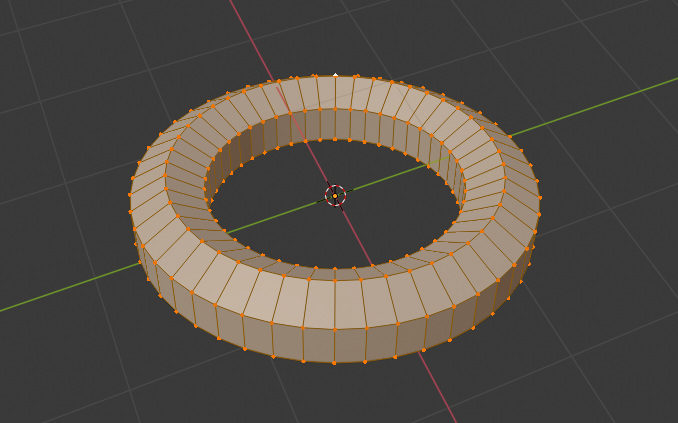
\includegraphics[width=0.4\textwidth]{blender_torus}
\caption{Primer modela v programu Blender.}
\end{figure}
  
Imeli smo učno in testno množico. Razlike med učnimi in testnimi modeli so bile v velikosti, poziciji in rotaciji.

\section{Metode}

\subsection{Trajnostna topologija}

Def: .method for computing topological features of a space at different spatial resolutions. More persistent features are detected over a wide range of spatial scales and are deemed more likely to represent true features of the underlying space rather than artifacts of sampling, noise, or particular choice of parameters


Intro:

To so disk, črta, krožnica, sfera in torus. Te oblike po večini spadajo v različne homološke grupe, zato smo iskali postopek za določanje homoloških grup. Odločili smo se za izgradnjo kompleksov in računanje Betti števil pri različnih razdaljah med točkami. Na podlagi spreminjanja stevila komponent v prvih treh dimenzijah smo nato določili homološko grupo. 


Izbira epsilona, vietoris rips

Izdelava Vietoris-Rips kompleksa
Granna

\subsection{Betti numbers}
Računanje
Treshold

Problem prepoznavanja modelov iz izte homološke grupe.

\subsection{Prepoznavanje modelov iz ste homološke grupe}

Za prepoznavanje 

\section{Rešitve}
% slike betti

Rezultati

% slike rezultati

\section{Zaključek}

Izboljšave:
- Učinkovitejši uzračun kompleksov-recimo alpha shape, da ma betti manj dela

Treshold za betti v splošnem malo drugačen


\end{document}


